\documentclass[1p]{elsarticle_modified}
%\bibliographystyle{elsarticle-num}

%\usepackage[colorlinks]{hyperref}
%\usepackage{abbrmath_seonhwa} %\Abb, \Ascr, \Acal ,\Abf, \Afrak
\usepackage{amsfonts}
\usepackage{amssymb}
\usepackage{amsmath}
\usepackage{amsthm}
\usepackage{scalefnt}
\usepackage{amsbsy}
\usepackage{kotex}
\usepackage{caption}
\usepackage{subfig}
\usepackage{color}
\usepackage{graphicx}
\usepackage{xcolor} %% white, black, red, green, blue, cyan, magenta, yellow
\usepackage{float}
\usepackage{setspace}
\usepackage{hyperref}

\usepackage{tikz}
\usetikzlibrary{arrows}

\usepackage{multirow}
\usepackage{array} % fixed length table
\usepackage{hhline}

%%%%%%%%%%%%%%%%%%%%%
\makeatletter
\renewcommand*\env@matrix[1][\arraystretch]{%
	\edef\arraystretch{#1}%
	\hskip -\arraycolsep
	\let\@ifnextchar\new@ifnextchar
	\array{*\c@MaxMatrixCols c}}
\makeatother %https://tex.stackexchange.com/questions/14071/how-can-i-increase-the-line-spacing-in-a-matrix
%%%%%%%%%%%%%%%

\usepackage[normalem]{ulem}

\newcommand{\msout}[1]{\ifmmode\text{\sout{\ensuremath{#1}}}\else\sout{#1}\fi}
%SOURCE: \msout is \stkout macro in https://tex.stackexchange.com/questions/20609/strikeout-in-math-mode

\newcommand{\cancel}[1]{
	\ifmmode
	{\color{red}\msout{#1}}
	\else
	{\color{red}\sout{#1}}
	\fi
}

\newcommand{\add}[1]{
	{\color{blue}\uwave{#1}}
}

\newcommand{\replace}[2]{
	\ifmmode
	{\color{red}\msout{#1}}{\color{blue}\uwave{#2}}
	\else
	{\color{red}\sout{#1}}{\color{blue}\uwave{#2}}
	\fi
}

\newcommand{\Sol}{\mathcal{S}} %segment
\newcommand{\D}{D} %diagram
\newcommand{\A}{\mathcal{A}} %arc


%%%%%%%%%%%%%%%%%%%%%%%%%%%%%5 test

\def\sl{\operatorname{\textup{SL}}(2,\Cbb)}
\def\psl{\operatorname{\textup{PSL}}(2,\Cbb)}
\def\quan{\mkern 1mu \triangleright \mkern 1mu}

\theoremstyle{definition}
\newtheorem{thm}{Theorem}[section]
\newtheorem{prop}[thm]{Proposition}
\newtheorem{lem}[thm]{Lemma}
\newtheorem{ques}[thm]{Question}
\newtheorem{cor}[thm]{Corollary}
\newtheorem{defn}[thm]{Definition}
\newtheorem{exam}[thm]{Example}
\newtheorem{rmk}[thm]{Remark}
\newtheorem{alg}[thm]{Algorithm}

\newcommand{\I}{\sqrt{-1}}
\begin{document}

%\begin{frontmatter}
%
%\title{Boundary parabolic representations of knots up to 8 crossings}
%
%%% Group authors per affiliation:
%\author{Yunhi Cho} 
%\address{Department of Mathematics, University of Seoul, Seoul, Korea}
%\ead{yhcho@uos.ac.kr}
%
%
%\author{Seonhwa Kim} %\fnref{s_kim}}
%\address{Center for Geometry and Physics, Institute for Basic Science, Pohang, 37673, Korea}
%\ead{ryeona17@ibs.re.kr}
%
%\author{Hyuk Kim}
%\address{Department of Mathematical Sciences, Seoul National University, Seoul 08826, Korea}
%\ead{hyukkim@snu.ac.kr}
%
%\author{Seokbeom Yoon}
%\address{Department of Mathematical Sciences, Seoul National University, Seoul, 08826,  Korea}
%\ead{sbyoon15@snu.ac.kr}
%
%\begin{abstract}
%We find all boundary parabolic representation of knots up to 8 crossings.
%
%\end{abstract}
%\begin{keyword}
%    \MSC[2010] 57M25 
%\end{keyword}
%
%\end{frontmatter}

%\linenumbers
%\tableofcontents
%
\newcommand\colored[1]{\textcolor{white}{\rule[-0.35ex]{0.8em}{1.4ex}}\kern-0.8em\color{red} #1}%
%\newcommand\colored[1]{\textcolor{white}{ #1}\kern-2.17ex	\textcolor{white}{ #1}\kern-1.81ex	\textcolor{white}{ #1}\kern-2.15ex\color{red}#1	}

{\Large $\underline{10_{25}~(K10a_{61})}$}

\setlength{\tabcolsep}{10pt}
\renewcommand{\arraystretch}{1.6}
\vspace{1cm}\begin{tabular}{m{100pt}>{\centering\arraybackslash}m{274pt}}
\multirow{5}{120pt}{
	\centering
	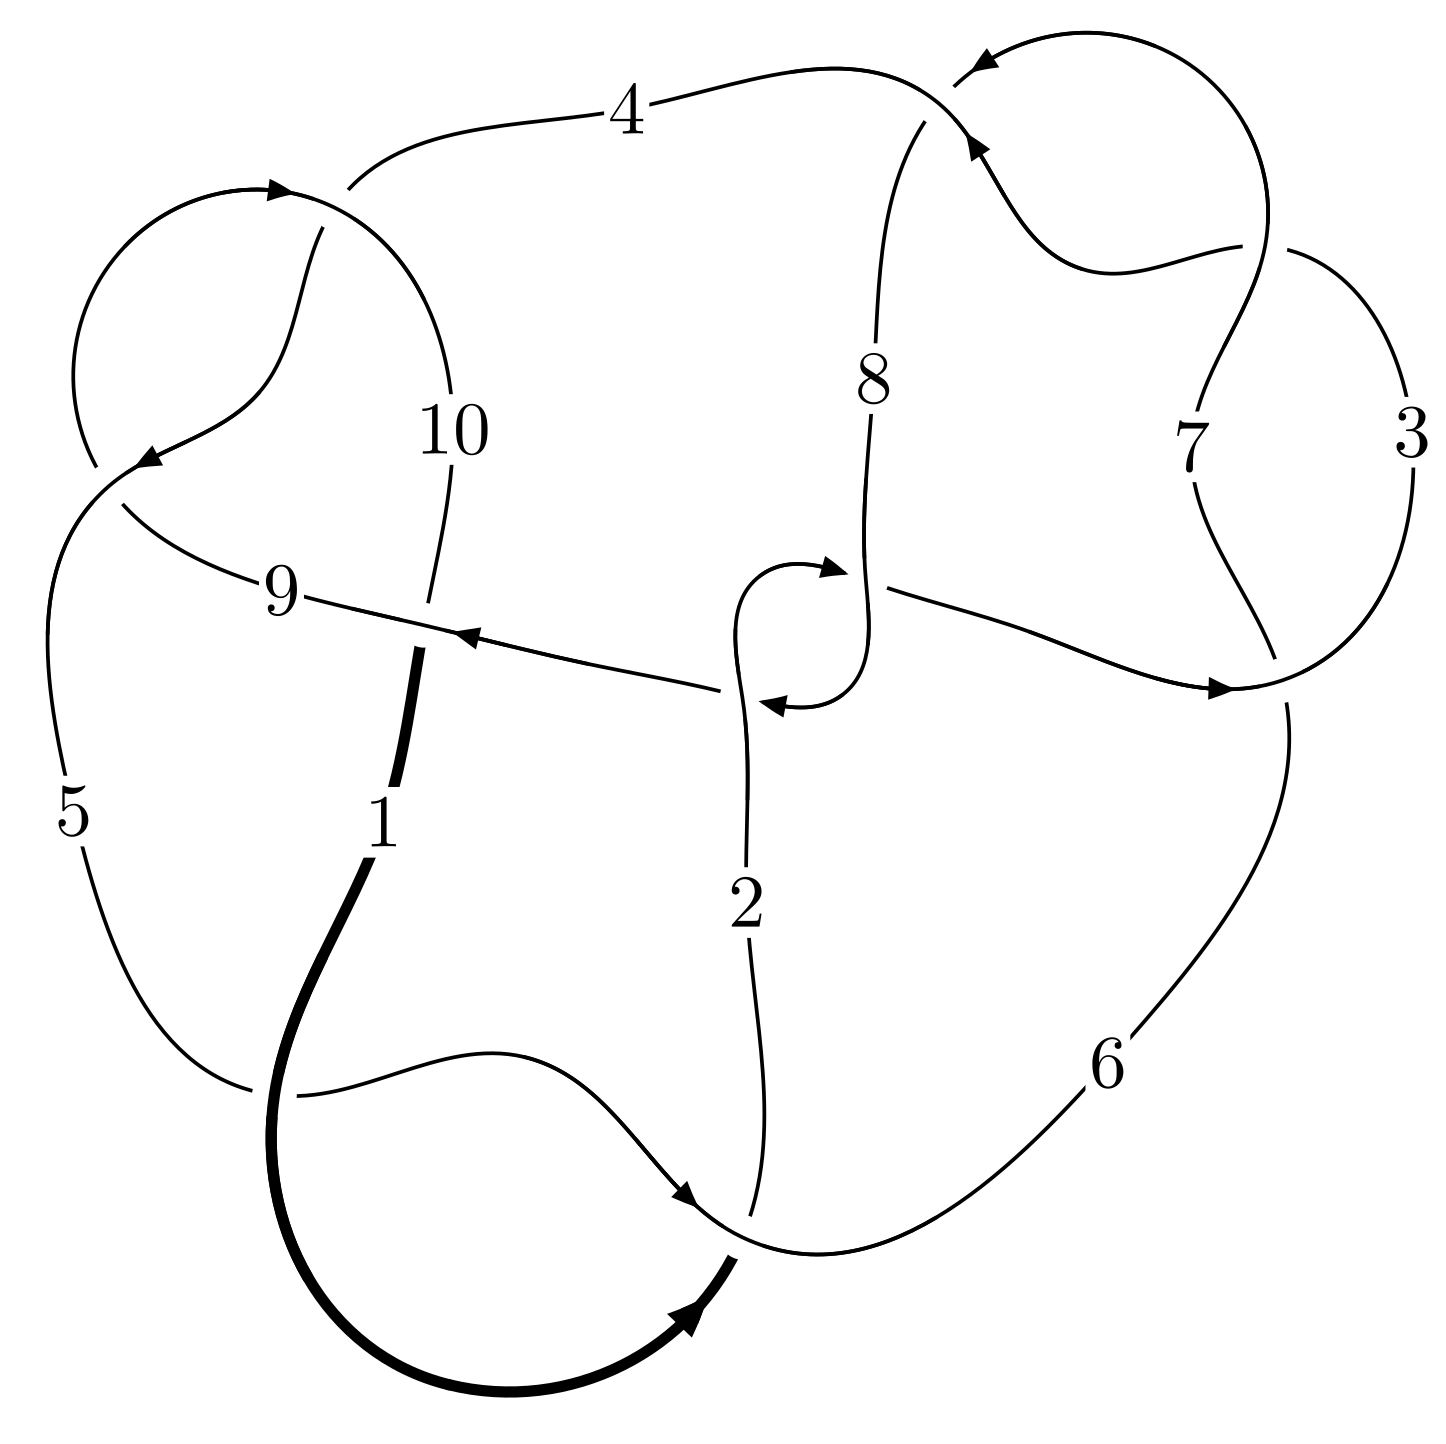
\includegraphics[width=112pt]{../../../GIT/diagram.site/Diagrams/png/109_10_25.png}\\
\ \ \ A knot diagram\footnotemark}&
\allowdisplaybreaks
\textbf{Linearized knot diagam} \\
\cline{2-2}
 &
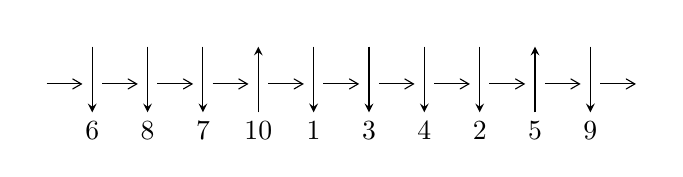
\begin{tikzpicture}[x=20pt, y=17pt]
	% nodes
	\node (C0) at (0, 0) {};
	\node (C1) at (1, 0) {};
	\node (C1U) at (1, +1) {};
	\node (C1D) at (1, -1) {6};

	\node (C2) at (2, 0) {};
	\node (C2U) at (2, +1) {};
	\node (C2D) at (2, -1) {8};

	\node (C3) at (3, 0) {};
	\node (C3U) at (3, +1) {};
	\node (C3D) at (3, -1) {7};

	\node (C4) at (4, 0) {};
	\node (C4U) at (4, +1) {};
	\node (C4D) at (4, -1) {10};

	\node (C5) at (5, 0) {};
	\node (C5U) at (5, +1) {};
	\node (C5D) at (5, -1) {1};

	\node (C6) at (6, 0) {};
	\node (C6U) at (6, +1) {};
	\node (C6D) at (6, -1) {3};

	\node (C7) at (7, 0) {};
	\node (C7U) at (7, +1) {};
	\node (C7D) at (7, -1) {4};

	\node (C8) at (8, 0) {};
	\node (C8U) at (8, +1) {};
	\node (C8D) at (8, -1) {2};

	\node (C9) at (9, 0) {};
	\node (C9U) at (9, +1) {};
	\node (C9D) at (9, -1) {5};

	\node (C10) at (10, 0) {};
	\node (C10U) at (10, +1) {};
	\node (C10D) at (10, -1) {9};
	\node (C11) at (11, 0) {};

	% arrows
	\draw[->,>={angle 60}]
	(C0) edge (C1) (C1) edge (C2) (C2) edge (C3) (C3) edge (C4) (C4) edge (C5) (C5) edge (C6) (C6) edge (C7) (C7) edge (C8) (C8) edge (C9) (C9) edge (C10) (C10) edge (C11) ;	\draw[->,>=stealth]
	(C1U) edge (C1D) (C2U) edge (C2D) (C3U) edge (C3D) (C4D) edge (C4U) (C5U) edge (C5D) (C6U) edge (C6D) (C7U) edge (C7D) (C8U) edge (C8D) (C9D) edge (C9U) (C10U) edge (C10D) ;
	\end{tikzpicture} \\
\hhline{~~} \\& 
\textbf{Solving Sequence} \\ \cline{2-2} 
 &
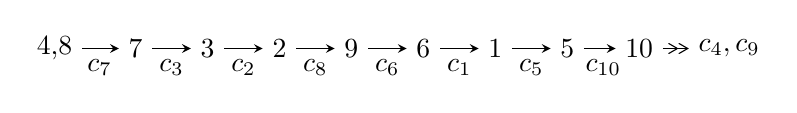
\begin{tikzpicture}[x=26pt, y=7pt]
	% node
	\node (A0) at (-1/8, 0) {4,8};
	\node (A1) at (1, 0) {7};
	\node (A2) at (2, 0) {3};
	\node (A3) at (3, 0) {2};
	\node (A4) at (4, 0) {9};
	\node (A5) at (5, 0) {6};
	\node (A6) at (6, 0) {1};
	\node (A7) at (7, 0) {5};
	\node (A8) at (8, 0) {10};
	\node (C1) at (1/2, -1) {$c_{7}$};
	\node (C2) at (3/2, -1) {$c_{3}$};
	\node (C3) at (5/2, -1) {$c_{2}$};
	\node (C4) at (7/2, -1) {$c_{8}$};
	\node (C5) at (9/2, -1) {$c_{6}$};
	\node (C6) at (11/2, -1) {$c_{1}$};
	\node (C7) at (13/2, -1) {$c_{5}$};
	\node (C8) at (15/2, -1) {$c_{10}$};
	\node (A9) at (37/4, 0) {$c_{4},c_{9}$};

	% edge
	\draw[->,>=stealth]	
	(A0) edge (A1) (A1) edge (A2) (A2) edge (A3) (A3) edge (A4) (A4) edge (A5) (A5) edge (A6) (A6) edge (A7) (A7) edge (A8) ;
	\draw[->>,>={angle 60}]	
	(A8) edge (A9);
\end{tikzpicture} \\ 

\end{tabular} \\

\footnotetext{
The image of knot diagram is generated by the software ``\textbf{Draw programme}" developed by Andrew Bartholomew(\url{http://www.layer8.co.uk/maths/draw/index.htm\#Running-draw}), where we modified some parts for our purpose(\url{https://github.com/CATsTAILs/LinksPainter}).
}\phantom \\ \newline 
\centering \textbf{Ideals for irreducible components\footnotemark of $X_{\text{par}}$} 
 
\begin{align*}
I^u_{1}&=\langle 
u^{32}+u^{31}+\cdots-2 u-1\rangle \\
\\
\end{align*}
\raggedright * 1 irreducible components of $\dim_{\mathbb{C}}=0$, with total 32 representations.\\
\footnotetext{All coefficients of polynomials are rational numbers. But the coefficients are sometimes approximated in decimal forms when there is not enough margin.}
\newpage
\renewcommand{\arraystretch}{1}
\centering \section*{I. $I^u_{1}= \langle u^{32}+u^{31}+\cdots-2 u-1 \rangle$}
\flushleft \textbf{(i) Arc colorings}\\
\begin{tabular}{m{7pt} m{180pt} m{7pt} m{180pt} }
\flushright $a_{4}=$&$\begin{pmatrix}0\\u\end{pmatrix}$ \\
\flushright $a_{8}=$&$\begin{pmatrix}1\\0\end{pmatrix}$ \\
\flushright $a_{7}=$&$\begin{pmatrix}1\\- u^2\end{pmatrix}$ \\
\flushright $a_{3}=$&$\begin{pmatrix}u\\- u^3+u\end{pmatrix}$ \\
\flushright $a_{2}=$&$\begin{pmatrix}- u^3+2 u\\- u^3+u\end{pmatrix}$ \\
\flushright $a_{9}=$&$\begin{pmatrix}u^6-3 u^4+2 u^2+1\\u^6-2 u^4+u^2\end{pmatrix}$ \\
\flushright $a_{6}=$&$\begin{pmatrix}- u^2+1\\u^4-2 u^2\end{pmatrix}$ \\
\flushright $a_{1}=$&$\begin{pmatrix}- u^9+4 u^7-5 u^5+3 u\\u^{11}-5 u^9+8 u^7-3 u^5-3 u^3+u\end{pmatrix}$ \\
\flushright $a_{5}=$&$\begin{pmatrix}u^{16}-7 u^{14}+19 u^{12}-22 u^{10}+3 u^8+14 u^6-6 u^4-4 u^2+1\\- u^{18}+8 u^{16}-25 u^{14}+36 u^{12}-17 u^{10}-12 u^8+12 u^6+2 u^4-3 u^2\end{pmatrix}$ \\
\flushright $a_{10}=$&$\begin{pmatrix}u^{23}-10 u^{21}+\cdots-2 u^3+4 u\\u^{23}-9 u^{21}+\cdots-2 u^3+u\end{pmatrix}$\\&\end{tabular}
\flushleft \textbf{(ii) Obstruction class $= -1$}\\~\\
\flushleft \textbf{(iii) Cusp Shapes $= -4 u^{29}+48 u^{27}-4 u^{26}-252 u^{25}+44 u^{24}+740 u^{23}-208 u^{22}-1264 u^{21}+536 u^{20}+1080 u^{19}-768 u^{18}+64 u^{17}+480 u^{16}-1008 u^{15}+176 u^{14}+612 u^{13}-436 u^{12}+320 u^{11}+120 u^{10}-424 u^9+128 u^8-4 u^7-60 u^6+108 u^5-12 u^4-4 u^3+4 u^2-12 u-10$}\\~\\
\newpage\renewcommand{\arraystretch}{1}
\flushleft \textbf{(iv) u-Polynomials at the component}\newline \\
\begin{tabular}{m{50pt}|m{274pt}}
Crossings & \hspace{64pt}u-Polynomials at each crossing \\
\hline $$\begin{aligned}c_{1},c_{5}\end{aligned}$$&$\begin{aligned}
&u^{32}- u^{31}+\cdots+14 u-5
\end{aligned}$\\
\hline $$\begin{aligned}c_{2},c_{8}\end{aligned}$$&$\begin{aligned}
&u^{32}-3 u^{31}+\cdots-4 u^4+1
\end{aligned}$\\
\hline $$\begin{aligned}c_{3},c_{6},c_{7}\end{aligned}$$&$\begin{aligned}
&u^{32}+u^{31}+\cdots-2 u-1
\end{aligned}$\\
\hline $$\begin{aligned}c_{4},c_{9}\end{aligned}$$&$\begin{aligned}
&u^{32}+u^{31}+\cdots-2 u-1
\end{aligned}$\\
\hline $$\begin{aligned}c_{10}\end{aligned}$$&$\begin{aligned}
&u^{32}+17 u^{31}+\cdots-8 u^2+1
\end{aligned}$\\
\hline
\end{tabular}\\~\\
\newpage\renewcommand{\arraystretch}{1}
\flushleft \textbf{(v) Riley Polynomials at the component}\newline \\
\begin{tabular}{m{50pt}|m{274pt}}
Crossings & \hspace{64pt}Riley Polynomials at each crossing \\
\hline $$\begin{aligned}c_{1},c_{5}\end{aligned}$$&$\begin{aligned}
&y^{32}-23 y^{31}+\cdots-296 y+25
\end{aligned}$\\
\hline $$\begin{aligned}c_{2},c_{8}\end{aligned}$$&$\begin{aligned}
&y^{32}+17 y^{31}+\cdots-8 y^2+1
\end{aligned}$\\
\hline $$\begin{aligned}c_{3},c_{6},c_{7}\end{aligned}$$&$\begin{aligned}
&y^{32}-27 y^{31}+\cdots+16 y^2+1
\end{aligned}$\\
\hline $$\begin{aligned}c_{4},c_{9}\end{aligned}$$&$\begin{aligned}
&y^{32}+17 y^{31}+\cdots-8 y^2+1
\end{aligned}$\\
\hline $$\begin{aligned}c_{10}\end{aligned}$$&$\begin{aligned}
&y^{32}-3 y^{31}+\cdots-16 y+1
\end{aligned}$\\
\hline
\end{tabular}\\~\\
\newpage\flushleft \textbf{(vi) Complex Volumes and Cusp Shapes}
$$\begin{array}{c|c|c}  
\text{Solutions to }I^u_{1}& \I (\text{vol} + \sqrt{-1}CS) & \text{Cusp shape}\\
 \hline 
\begin{aligned}
u &= \phantom{-}1.029010 + 0.281289 I\end{aligned}
 & -3.89830 + 3.89503 I & -9.35061 - 2.90091 I \\ \hline\begin{aligned}
u &= \phantom{-}1.029010 - 0.281289 I\end{aligned}
 & -3.89830 - 3.89503 I & -9.35061 + 2.90091 I \\ \hline\begin{aligned}
u &= -1.134230 + 0.236397 I\end{aligned}
 & -1.32933 + 0.52783 I & -5.59448 - 0.64788 I \\ \hline\begin{aligned}
u &= -1.134230 - 0.236397 I\end{aligned}
 & -1.32933 - 0.52783 I & -5.59448 + 0.64788 I \\ \hline\begin{aligned}
u &= \phantom{-}0.166316 + 0.775774 I\end{aligned}
 & -1.27472 - 7.88151 I & -6.19556 + 6.68910 I \\ \hline\begin{aligned}
u &= \phantom{-}0.166316 - 0.775774 I\end{aligned}
 & -1.27472 + 7.88151 I & -6.19556 - 6.68910 I \\ \hline\begin{aligned}
u &= \phantom{-}0.729645 + 0.240963 I\end{aligned}
 & -4.28206 - 3.88889 I & -10.89128 + 4.90467 I \\ \hline\begin{aligned}
u &= \phantom{-}0.729645 - 0.240963 I\end{aligned}
 & -4.28206 + 3.88889 I & -10.89128 - 4.90467 I \\ \hline\begin{aligned}
u &= -0.028912 + 0.764004 I\end{aligned}
 & \phantom{-}4.01456 + 2.24194 I & -0.65690 - 3.79727 I \\ \hline\begin{aligned}
u &= -0.028912 - 0.764004 I\end{aligned}
 & \phantom{-}4.01456 - 2.24194 I & -0.65690 + 3.79727 I \\ \hline\begin{aligned}
u &= -0.140851 + 0.748200 I\end{aligned}
 & \phantom{-}1.56622 + 3.15266 I & -2.67728 - 3.41480 I \\ \hline\begin{aligned}
u &= -0.140851 - 0.748200 I\end{aligned}
 & \phantom{-}1.56622 - 3.15266 I & -2.67728 + 3.41480 I \\ \hline\begin{aligned}
u &= \phantom{-}0.191682 + 0.700576 I\end{aligned}
 & -2.34434 + 0.39737 I & -7.83598 + 0.58140 I \\ \hline\begin{aligned}
u &= \phantom{-}0.191682 - 0.700576 I\end{aligned}
 & -2.34434 - 0.39737 I & -7.83598 - 0.58140 I \\ \hline\begin{aligned}
u &= -1.237710 + 0.313650 I\end{aligned}
 & \phantom{-}0.29651 + 1.65231 I & -4.59303 - 0.15309 I \\ \hline\begin{aligned}
u &= -1.237710 - 0.313650 I\end{aligned}
 & \phantom{-}0.29651 - 1.65231 I & -4.59303 + 0.15309 I \\ \hline\begin{aligned}
u &= \phantom{-}1.288430 + 0.161328 I\end{aligned}
 & -5.00599 - 2.81562 I & -13.51638 + 3.82546 I \\ \hline\begin{aligned}
u &= \phantom{-}1.288430 - 0.161328 I\end{aligned}
 & -5.00599 + 2.81562 I & -13.51638 - 3.82546 I \\ \hline\begin{aligned}
u &= \phantom{-}1.281200 + 0.325415 I\end{aligned}
 & -0.06115 - 6.17510 I & -5.73067 + 6.90538 I \\ \hline\begin{aligned}
u &= \phantom{-}1.281200 - 0.325415 I\end{aligned}
 & -0.06115 + 6.17510 I & -5.73067 - 6.90538 I \\ \hline\begin{aligned}
u &= \phantom{-}1.350330 + 0.317347 I\end{aligned}
 & -3.13584 - 7.01747 I & -7.66223 + 4.88322 I \\ \hline\begin{aligned}
u &= \phantom{-}1.350330 - 0.317347 I\end{aligned}
 & -3.13584 + 7.01747 I & -7.66223 - 4.88322 I \\ \hline\begin{aligned}
u &= \phantom{-}1.39424\phantom{ +0.000000I}\end{aligned}
 & -7.31963\phantom{ +0.000000I} & -11.4830\phantom{ +0.000000I} \\ \hline\begin{aligned}
u &= -1.364340 + 0.293820 I\end{aligned}
 & -7.25067 + 3.23058 I & -12.64791 - 1.85611 I \\ \hline\begin{aligned}
u &= -1.364340 - 0.293820 I\end{aligned}
 & -7.25067 - 3.23058 I & -12.64791 + 1.85611 I \\ \hline\begin{aligned}
u &= -0.599844\phantom{ +0.000000I}\end{aligned}
 & -1.22821\phantom{ +0.000000I} & -8.26170\phantom{ +0.000000I} \\ \hline\begin{aligned}
u &= -1.364190 + 0.328069 I\end{aligned}
 & -6.10646 + 11.87580 I & -10.77954 - 7.99531 I \\ \hline\begin{aligned}
u &= -1.364190 - 0.328069 I\end{aligned}
 & -6.10646 - 11.87580 I & -10.77954 + 7.99531 I \\ \hline\begin{aligned}
u &= -1.41547 + 0.02215 I\end{aligned}
 & -10.82670 + 4.39858 I & -14.8085 - 3.5355 I \\ \hline\begin{aligned}
u &= -1.41547 - 0.02215 I\end{aligned}
 & -10.82670 - 4.39858 I & -14.8085 + 3.5355 I\\
 \hline 
 \end{array}$$\newpage$$\begin{array}{c|c|c}  
\text{Solutions to }I^u_{1}& \I (\text{vol} + \sqrt{-1}CS) & \text{Cusp shape}\\
 \hline 
\begin{aligned}
u &= -0.248101 + 0.323031 I\end{aligned}
 & -0.501058 + 1.034980 I & -7.18759 - 6.41402 I \\ \hline\begin{aligned}
u &= -0.248101 - 0.323031 I\end{aligned}
 & -0.501058 - 1.034980 I & -7.18759 + 6.41402 I\\
 \hline 
 \end{array}$$\newpage
\newpage\renewcommand{\arraystretch}{1}
\centering \section*{ II. u-Polynomials}
\begin{tabular}{m{50pt}|m{274pt}}
Crossings & \hspace{64pt}u-Polynomials at each crossing \\
\hline $$\begin{aligned}c_{1},c_{5}\end{aligned}$$&$\begin{aligned}
&u^{32}- u^{31}+\cdots+14 u-5
\end{aligned}$\\
\hline $$\begin{aligned}c_{2},c_{8}\end{aligned}$$&$\begin{aligned}
&u^{32}-3 u^{31}+\cdots-4 u^4+1
\end{aligned}$\\
\hline $$\begin{aligned}c_{3},c_{6},c_{7}\end{aligned}$$&$\begin{aligned}
&u^{32}+u^{31}+\cdots-2 u-1
\end{aligned}$\\
\hline $$\begin{aligned}c_{4},c_{9}\end{aligned}$$&$\begin{aligned}
&u^{32}+u^{31}+\cdots-2 u-1
\end{aligned}$\\
\hline $$\begin{aligned}c_{10}\end{aligned}$$&$\begin{aligned}
&u^{32}+17 u^{31}+\cdots-8 u^2+1
\end{aligned}$\\
\hline
\end{tabular}\newpage\renewcommand{\arraystretch}{1}
\centering \section*{ III. Riley Polynomials}
\begin{tabular}{m{50pt}|m{274pt}}
Crossings & \hspace{64pt}Riley Polynomials at each crossing \\
\hline $$\begin{aligned}c_{1},c_{5}\end{aligned}$$&$\begin{aligned}
&y^{32}-23 y^{31}+\cdots-296 y+25
\end{aligned}$\\
\hline $$\begin{aligned}c_{2},c_{8}\end{aligned}$$&$\begin{aligned}
&y^{32}+17 y^{31}+\cdots-8 y^2+1
\end{aligned}$\\
\hline $$\begin{aligned}c_{3},c_{6},c_{7}\end{aligned}$$&$\begin{aligned}
&y^{32}-27 y^{31}+\cdots+16 y^2+1
\end{aligned}$\\
\hline $$\begin{aligned}c_{4},c_{9}\end{aligned}$$&$\begin{aligned}
&y^{32}+17 y^{31}+\cdots-8 y^2+1
\end{aligned}$\\
\hline $$\begin{aligned}c_{10}\end{aligned}$$&$\begin{aligned}
&y^{32}-3 y^{31}+\cdots-16 y+1
\end{aligned}$\\
\hline
\end{tabular}
\vskip 2pc
\end{document}